\documentclass{article}
\usepackage{graphicx} % Required for inserting images
\usepackage{amssymb}
\usepackage{listings}

\title{hetFL}
\author{shamsiiat.abdurakhmanova }
\date{February 2023}

\begin{document}

\maketitle

\section{Numerical experiments}

\subsection{Datasets}

\subsubsection{Synthetic Dataset}

Experiments were performed on a synthetic dataset whose empirical graph $\mathcal {G}$ is partitioned into 3 equal-sized clusters $\mathcal{P} = \{\mathcal{C}^{(1)}, \mathcal{C}^{(2)}, \mathcal{C}^{(3)}\}$, with $|\mathcal{C}^{(1)}|=|\mathcal{C}^{(2)}|=|\mathcal{C}^{(3)}|$. We denote the cluster assignment of node $i \in \mathcal{V}$ by ${c}^{(i)} \in \{1,2,3\}$. The edges in $\mathcal {G}$  are generated via realizations of independent binary random variables ${b}_{i,{i}^{'}} \in \{0,1\}$. These random variables are indexed by pairs $i,{i}^{'}$ of nodes that are connected by an edge $\{i,{i}^{'}\} \in \mathcal{E}$ if and only if ${b}_{i,{i}^{'}}=1$. \\
Two nodes in the same cluster are connected with probability $Prob\{{b}_{i,{i}^{'}}=1\} :={p}_{in}$ if nodes $i,{i}^{'}$ belong to the same cluster. In contrast, $Prob\{{b}_{i,{i}^{'}}=1\} :={p}_{out}$ if nodes $i,{i}^{'}$ belong to different clusters. Every edge in  $\mathcal {G}$ has the same weight, ${A}_{e}=1$ for all $e \in \mathcal{E}$.

Each node $i \in \mathcal {V}$ of the empirical graph $\mathcal {G}$ holds a local dataset $\mathcal {D}^{(i)}$ of the form $\mathcal {D}^{(i)} := \{ ({x}^{(i,1)}, {y}^{(i,1)}), ..., ({x}^{(i,{m}_{i})}, {y}^{(i,{m}_{i})}) \}$. Thus, dataset $\mathcal {D}_{(i)}$ consist of ${m}_{i}$ data points, each characterized by a feature vector $\mathbf{x}^{(i,r)} \in \mathbb{R}^{d}$ and scalar label ${y}^{(i,r)}$, for $r=1,...,{m}_{i}$. The feature vectors $\mathbf{x}^{(i,r)} \sim \mathcal{N}(\mathbf{0},\mathbf{I}_{d \times d})$, are drawn i.i.d. from a standard multivariate normal distribution. 

The labels of the data points are generated by a noisy linear model
\begin{equation}
{y}^{(i,r)} = (\mathbf{w}^{(i)})^T\mathbf{x}^{(i,r)} + {\varepsilon}^{(i,r)}
\end{equation}

The noise ${\varepsilon}^{(i,r)} \sim \mathcal{N}(0, 1)$, for $i \in \mathcal{V}$ and $r=1,..,{m}_{i}$, are i.i.d. realizations of a normal distribution. The true underlying vector $\mathbf{w}^{(i)} \sim \mathcal{N}(0,1)$ is drawn from a standard normal distribution and is the same for nodes from the same cluster, i.e. $\mathbf{w}^{(i)}=\mathbf{w}^{({i}^{'})}$ if ${c}^{(i)}={c}^{({i}^{'})}$.

Datasets were divided into training and validation subsets by using resampling with replacement. The size of the validation subset was ${m}^{(val)}_{i}=100$. 

\subsubsection{Shared Dataset}

Dataset $\mathcal{D}^{(test)}$, which predictions are shared across all nodes was formed as follows:
the feature, weight and noise vectors are drawn i.i.d. from a standard normal distribution and labels are generated by a noisy linear model. The size of the dataset was $m'=100$. 

\subsection{Experiments}
In these experiments empirical graph $\mathcal{G}$ consist of 15 nodes partitioned into three clusters. Two nodes in the same cluster are connected with probability ${p}_{in}=0.8$ if nodes $i,{i}^{'}$ belong to the same cluster and ${p}_{out}=0.2$ if nodes $i,{i}^{'}$ belong to different clusters. 

Each node $i \in \mathcal {V}$ of the empirical graph $\mathcal {G}$ holds a local dataset $\mathcal{D}^{(i)}$ consisting of ${m}_{i}$ data points, each characterized by a feature vector $\mathbf{x}^{(i,r)} \in \mathbb{R}^{d}$ and scalar label ${y}^{(i,r)}$, for $r=1,...,{m}_{i}$, where $d=10$.
The sample size of the shared dataset $\mathcal{D}^{(test)}$ is ${m}^{'}=100$.

To learn the local parameters $\mathbf{w}^{(i)}$, we use Algorithm 2 with local loss 

\begin{equation}
{L}_{(i)}({h}^{(i)}) = \frac{1}{{m}_{i}} \sum_{r=1}^{{m}_{i}}\left({y}^{(i,r)} - {h}^{(i)}(\mathbf{x}^{(i,r)}) \right)^2
\end{equation}

and  regularizer 

\begin{equation}
\frac{\lambda}{{2m}^{'}} \sum_{{i}^{'} \in {\mathcal V}} {A}_{i,{i}^{'}} \sum_{r=1}^{{m}^{'}} \left({h}^{(i)}(\mathbf{x}^{(r)}) - {h}^{({i}^{'})}(\mathbf{x}^{(r)}) \right)^2
\end{equation}

As stopping criterion in Algorithm 2, we use a fixed number of R = 1000 iterations. 

Below we plot average training and validation MSE of all nodes over 10 runs. On each run new local $\mathcal{D}^{(i)}$ and shared $\mathcal{D}^{(test)}$ datasets were generated. The error bar is one standard deviation (lower limit is omitted for clarity).  

Results on the synthetic datasets:

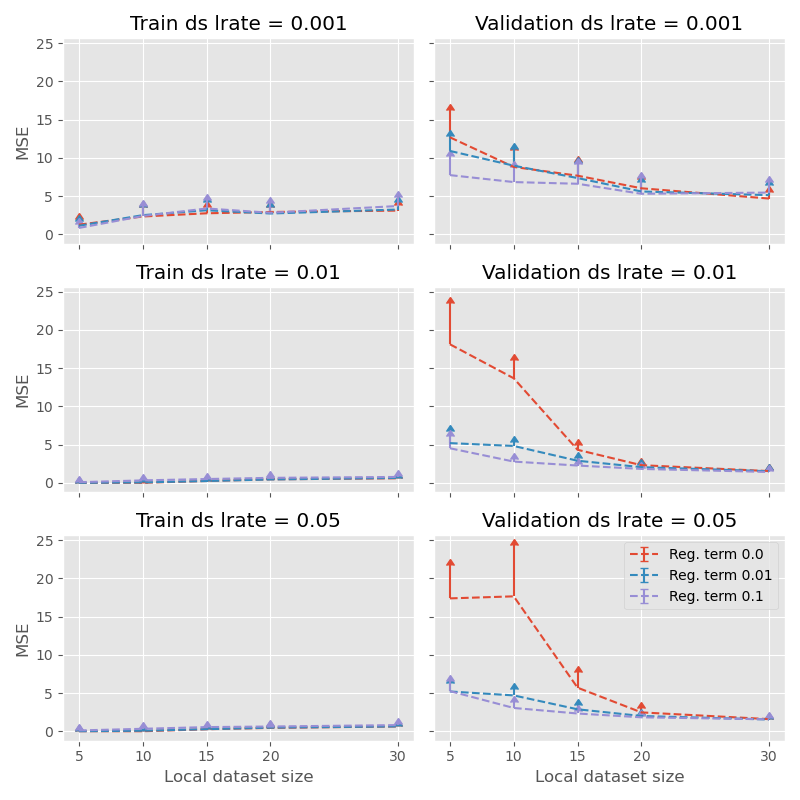
\includegraphics[width=10cm]{linreg_syn_I_ds_lrate.png}


\end{document}
